% $Id: INF_Poster.tex 7714 2011-08-31 17:34:46Z tkren $
%
% TU Wien - Faculty of Informatics
% poster template
%
% This template is using the beamer document class and beamerposter package, see
% <http://www.ctan.org/tex-archive/macros/latex/contrib/beamer/>
% <http://www.ctan.org/tex-archive/macros/latex/contrib/beamerposter/>
% <http://www-i6.informatik.rwth-aachen.de/~dreuw/latexbeamerposter.php>
%
% For questions and comments send an email to
% Thomas Krennwallner <tkren@kr.tuwien.ac.at>
%

\documentclass[final,hyperref={pdfpagelabels=false}]{beamer}

\usepackage{TUINFPST}

\title[Computational Intelligence]{Design and Implementation of an Agent Architecture combining Emotions and Reasoning}
\author[janos.tapolczai@alumni.tuwien.ac.at]{Janos Tapolczai}
\institute[]{%
    Technische Universit{\"a}t Wien\\[0.25\baselineskip]
    Institut f{\"u}r Informationssysteme 184/3\\[0.25\baselineskip]
    Arbeitsbereich: Knowledge Based Systems\\[0.25\baselineskip]
    BetreuerIn: a.o. Univ.-Prof. Dr. Hans Tompits\\[0.25\baselineskip]
}
\titlegraphic{
\includegraphics[height=52mm]{kbs-logo}}
\date[\today]{\today}
\subject{epilog}
\keywords{artificial intelligence, reasoning, affective}

%%%%%%%%%%%%%%%%%%%%%%%%%%%%%%%%%%%%%%%%%%%%%%%%%%%%%%%%%%%%%%%%%%%%%%%%%%%%%%%%%%%%%%
% Display a grid to help align images 
%\beamertemplategridbackground[1cm]

% play around with the background colors
% \setbeamercolor{background canvas}{bg=yellow}

% use a background picture
% \usebackgroundtemplate{%
%   
\includegraphics[width=\paperwidth]{logo_KBS_2_CMYK}
% }

% play around with block colors
\setbeamercolor{block body}{fg=black,bg=white}
\setbeamercolor{block title}{fg=TuWienBlue,bg=white}

\setbeamertemplate{block begin}{
    \begin{beamercolorbox}{block title}%
        
\begin{tikzpicture}%
        \node[draw,rectangle,line width=3pt,rounded corners=0pt,inner sep=0pt]{%
            \begin{minipage}[c][2cm]{\linewidth}
            \centering\textbf{\insertblocktitle}
            \end{minipage}
        };
        \end{tikzpicture}%
    \end{beamercolorbox}
    \vspace*{1cm}
    \begin{beamercolorbox}{block body}%
}
    
\setbeamertemplate{block end}{
    \end{beamercolorbox}
    \vspace{2cm}
}

% setup postit
\setbeamercolor{postit}{fg=black,bg=yellow} 
\newenvironment{postit}
{\begin{beamercolorbox}[sep=1em,wd=7cm]{postit}}
{\end{beamercolorbox}}

% for crop marks, uncomment the following line
%\usepackage[cross,width=88truecm,height=123truecm,center]{crop}

% setup url size
\usepackage{url}
\urlstyle{same}

% setup download links
\usepackage{wrapfig}
\usepackage{qrcode}

% setup bibliography
\bibliographystyle{plain}

%%%%%%%%%%%%%%%%%%%%%%%%%%%%%%%%%%%%%%%%%%%%%%%%%%%%%%%%%%%%%%%%%%%%%%%%%%%%%%%%%%%%%%

\begin{document}

% We have a single poster frame.
\begin{frame}
    \begin{columns}[t]
        % ---------------------------------------------------------%
        % Set up a column
        \begin{column}{.45\textwidth}
            \begin{block}{Introduction \& Problem Statement}                
                \begin{itemize}
                    \item Reasoning and search can explore solution spaces, but they can't tell an agent which goals it should value.
                    \item Often, outcomes are valued via goal functions and are categorized into ``good'' and ``bad'' ones, depending on the value of the function.
                    \item Can one combine simple emotional reactions to situations with reasoning techniques to obtain intelligent behaviour?
                \end{itemize}
                
                $~$
                
                \textbf{Wumpus World}\\
                We set our agents in a 2D-grid world with predators that try to kill agents, plants that can be harvested. Agents have to avoid being killed and eat to survive.
            \end{block}
            
            \begin{block}{Combining Affect and Reasoning}                
                We have created an AI consisting of loosely coupled components that communicate via a central message space.
                
                $~$
                
                \textbf{Structure}
                \begin{itemize}
                	\item Agents emotionally evaluate their current situation and take a hypothetical action based on the strongest emotion.
                	\item The world is simulated one step ahead.
                	\item If the outcome satisfies the strongest emotion, the action is actually taken.
                	\item If not, the planning continues or a different action is tried.
                \end{itemize}
                
                $~$
                
                \textbf{Emotions}
                \begin{itemize}
                	\item Evolutionarily speaking, organisms felt fear and anger long before they felt social emotions.
                	\item We implemented four emotions: anger, fear, enthusiasm, contentment.
                	\item Anger: \textbf{negative} and \textbf{approach-related},
                	\item Fear: \textbf{negative} and \textbf{avoidance-related}.
                	\item Enthusiasm: \textbf{positive} and \textbf{approach-related},
                	\item Contentment: \textbf{positive} and \textbf{avoidance-related},\\ (the organism avoids action because its needs are met).
                \end{itemize}
                
                $~$
                
                \begin{figure}
                	\centering
                	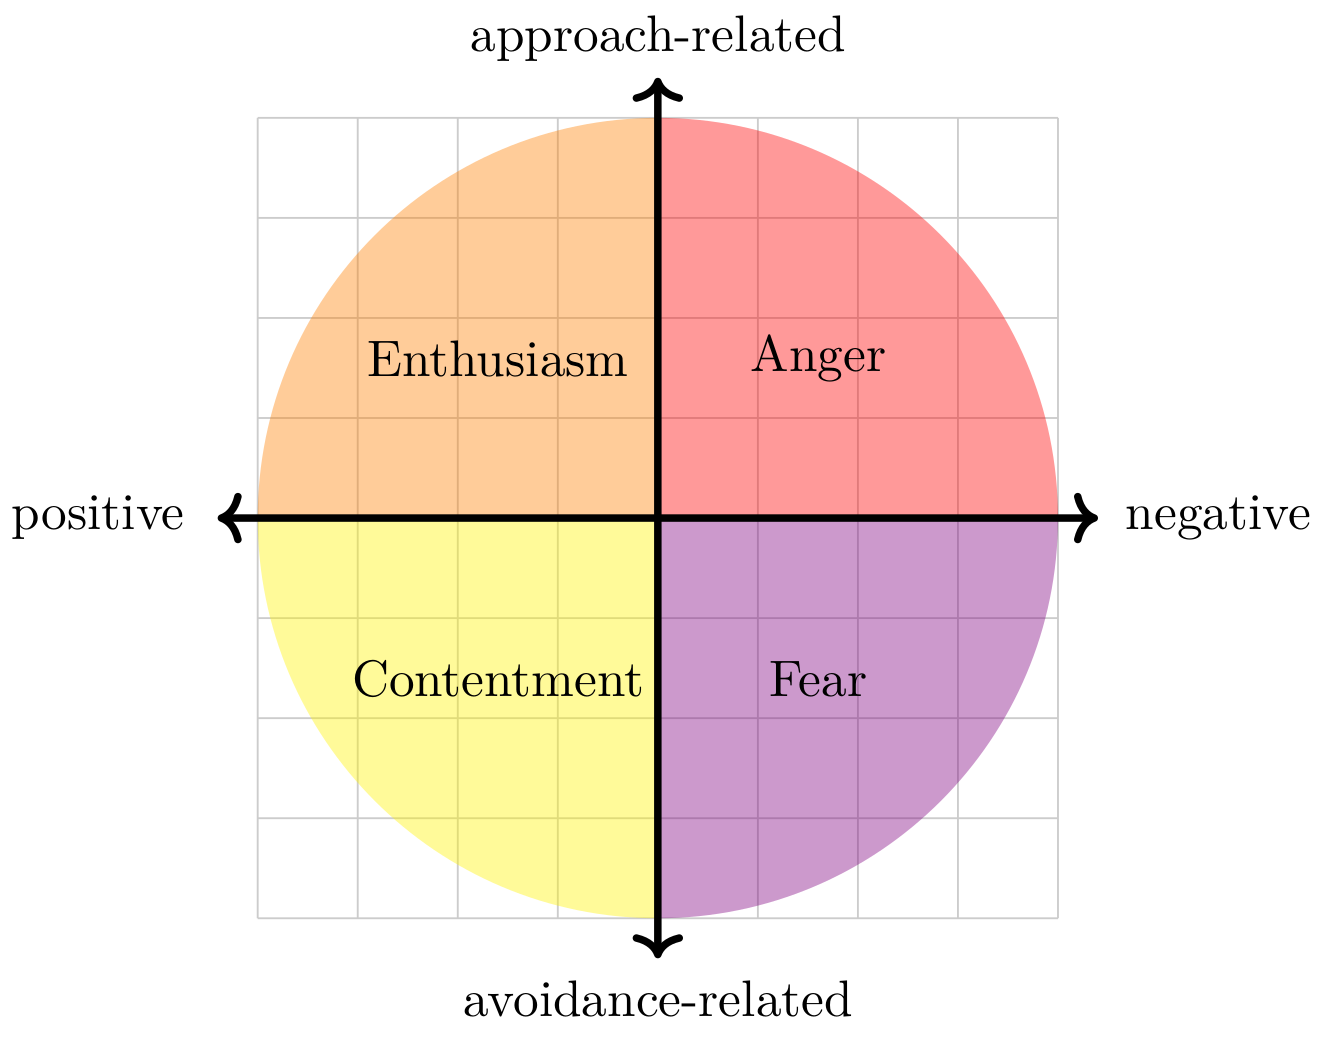
\includegraphics[width=0.75\textwidth]{figures/psbc.png}
                \end{figure}
            \end{block}
        \end{column}
        % ---------------------------------------------------------%
        % end the column
        
        % ---------------------------------------------------------%
        % Set up a column 
        \begin{column}{.45\textwidth}            
            \begin{block}{Proof of Concept}
            	We wrote a proof of the concept Haskell. The two major components are the world simulation and the AI.
                
                $~$
                
                \textbf{World simulation}
                \begin{itemize}
                    \item Implements the semantics of the Wumpus world.
                    \item Possible actions: rotate, move, pick up item, give item, attack, etc.
                    \item Agents get perceptions: visual data, breeze from pits, stench from predators, location, direction.
                    \item AIs are interfaces that implement a \texttt{getAction}-function.
                \end{itemize}
                
                $~$
                
                \textbf{AI}
                \begin{itemize}
                    \item Consists of loosely coupled components that communicate via a shared message space.
                    \item Components are called sequentially in each round.
                    \item Each component can read the previous messages and insert its own.
                    \item The pre-social behaviour control (PSBC) and social judgment system (SJS) provide emotional reactions.
                    \item The decision maker (DM) takes actions.
                    \item The belief generator (BG) simulates the consequences of actions.
                    \item The attention control (AC) selects important targets.
                \end{itemize}
                
                $~$
                
                \begin{figure}
                	\centering
                	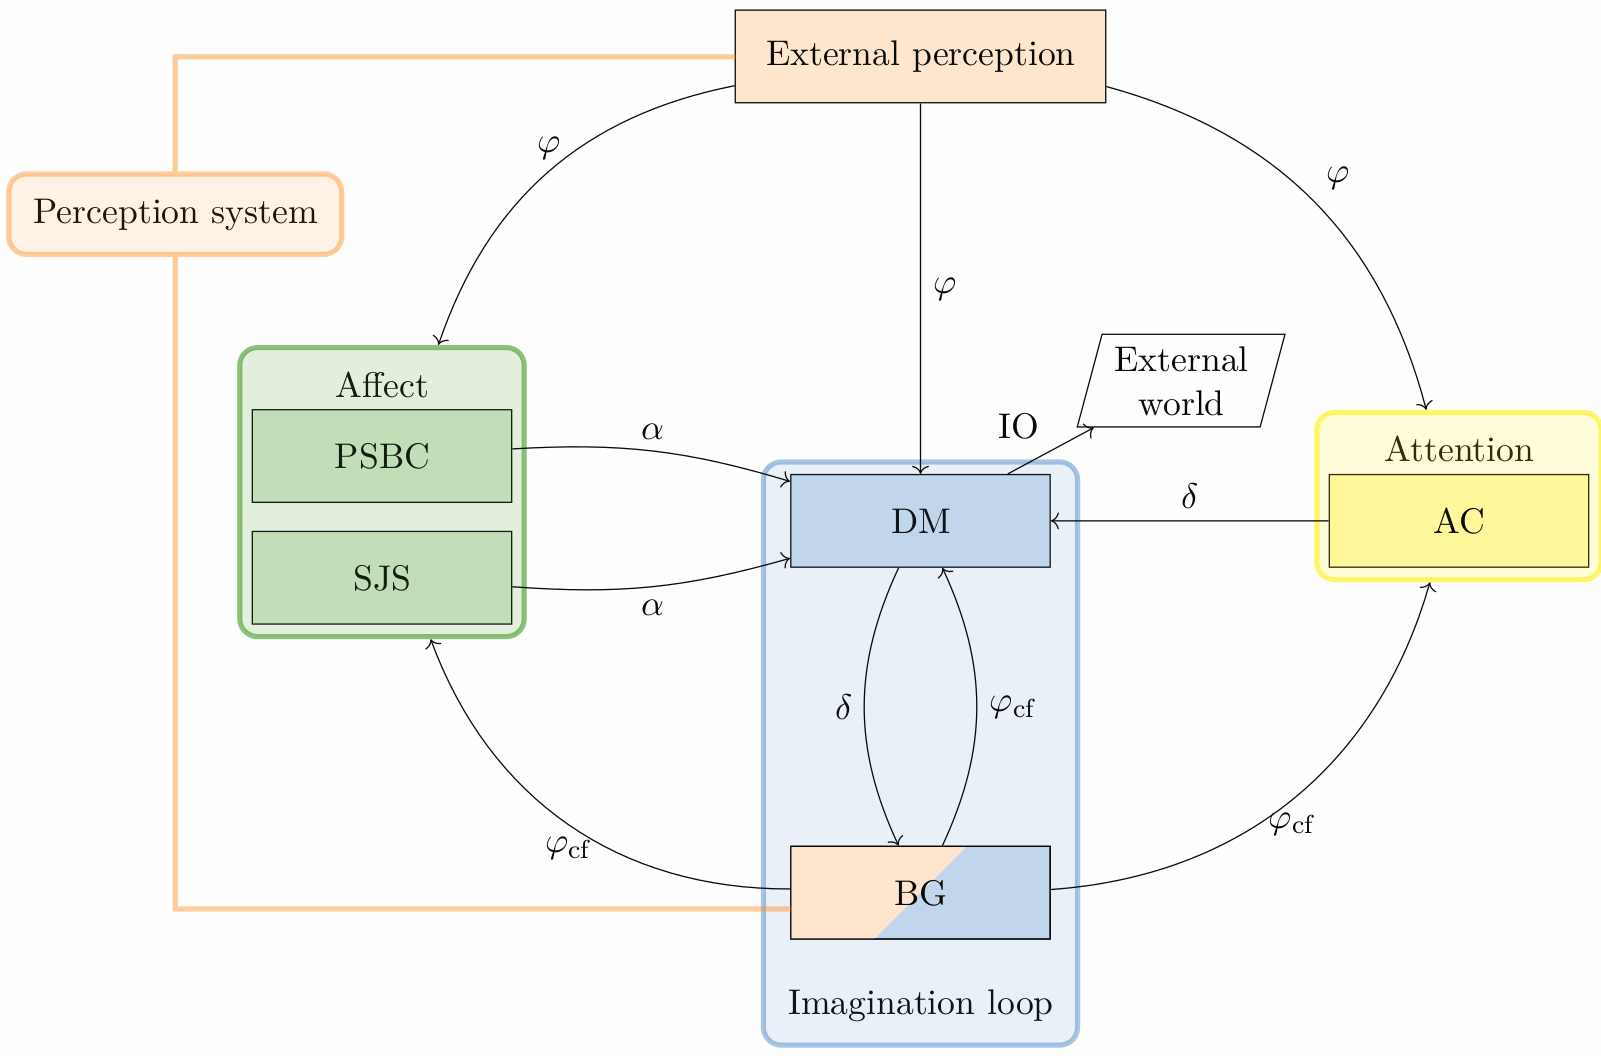
\includegraphics[width=0.75\textwidth]{figures/architecture.png}
                \end{figure}
            \end{block}
            
            \begin{block}{Evaluation}
                \begin{itemize}
                    \item The AIs had to perform tasks in simple test worlds (harvesting plants, fleeing, attacking weak enemies).
                    \item Different populations with different personalities were compared.
                \end{itemize}
            \end{block}
            
            \begin{block}{Conclusion}
                % use columns so we can print the download link to the right
                \begin{columns}[t]
                    \begin{column}{0.77\textwidth}
                        \begin{itemize}
                            \item We created a hybrid AI that combines emotions and reasoning.
                            \item There are no explicit goal functions, only conflicting emotions.
                            \item The AI performs well on simple tasks and in complex environments. Different personalities have different success rates.
                        \end{itemize}
                    \end{column}
                    % print the download link
                    \begin{column}{0.23\textwidth}
                        \begin{block}{DOWNLOAD}
                            \begin{center}
                                \qrcode[hyperlink,height=2.5in]{https://github.com/jtapolczai/wumpus}
                        \end{center}
                        \end{block}
                    \end{column}
                \end{columns}
            \end{block}
        \end{column}
        % ---------------------------------------------------------%
        % end the column
    \end{columns}
\end{frame}

\end{document}

%%% Local Variables:
%%% TeX-PDF-mode: t
%%% TeX-debug-bad-boxes: t
%%% TeX-master: t
%%% TeX-parse-self: t
%%% TeX-auto-save: t
%%% reftex-plug-into-AUCTeX: t
%%% End:
